We verify our algorithm GDSDA-SVM on the benchmark dataset Office. Moreover, we provide two different settings: single source and multi-source scenarios for GDSDA-SVM.
\subsection{Dataset}
There are 3 subsets in offices datasets, Webcam (795 examples), Amazon (2817 examples) and DSLR (498 examples), sharing 31 classes. In our experiments, we use DSLR and Webcam as the source domain and Amazon as the target domain.
We use the features extracted from Alexnet \cite{KrizhevskyNIPS12} FC7 as the input features for both source and target domain. The source model is trained with multi-layer perception (MLP) on the whole source dataset. 

\subsection{Single Source for Office datasets}
As we mentioned, there are significantly fewer labeled examples than unlabeled ones in real SDA applications. In this experiment, we compare our algorithm with the baselines in this situation where there is just one source model that generates the soft label. Specifically, we perform two groups of experiment using Amazon dataset as the target domain and DSLR and Webcam datasets as the source domain respectively. In each group of experiment, we show 3 results with different settings. We set the size of the labeled example to be 1 per class, and the size of the unlabeled example to be 10, 15 and 20 per class respectively.

To show the effectiveness of GDSDA-SVM, we also use brute force to search the imitation parameter $\lambda$ in the range $[0,0.1,...,1]$ with different temperature $T$ as the benchmark. We also show the performance of the source model on the target task, denoted as "Source" and the performance of a target model trained with only labeled examples in the target domain denoted as "No transfer". To avoid the randomness, we perform each experiment 10 times and report the average results. For GDSDA-SVM, we use temperature $T=20$. The experimental results are shown in Figure \ref{fig:single1}. 
%$\lambda$ on the X-axis of the figures denotes the imitation parameter for the hard label and the corresponding imitation parameter for the soft label is set to $1-\lambda$.

From the results of brutal force search, it is clear that the value of imitation parameter can greatly affect the performance of the target model.
Also, we can see that, when we only use the unlabeled data for distillation, i.e. $\lambda = 0$, as we expected, GDSDA can slightly outperform the source model. This means GDSDA can effectively transfer the knowledge between different domains with the unlabeled data. As we increase the value of imitation parameter, i.e. considering the hard labels from the target domain, the performance of GDSDA can be further improved. As we mentioned before, even though our "fake label" strategy would introduce extra noise, this noise can be limited by setting proper imitation parameter and the target model can still get improved performance compared to the model trained with ground truth labels (No transfer model in our experiment).
More importantly, we can see that the result of GDSDA-SVM can achieve the best performance in most of the situations compared to baselines using brutal force. This indicates that we can effectively (about 6 times times faster) obtain a good target model with our imitation parameter estimation method.
%\newpage
%\subsubsection{From DSLR to Amazon}
\begin{figure}[t]
\centering
\begin{tabular}{cccc}
\subfloat[D $\rightarrow$ A, 10 unlabeled ]{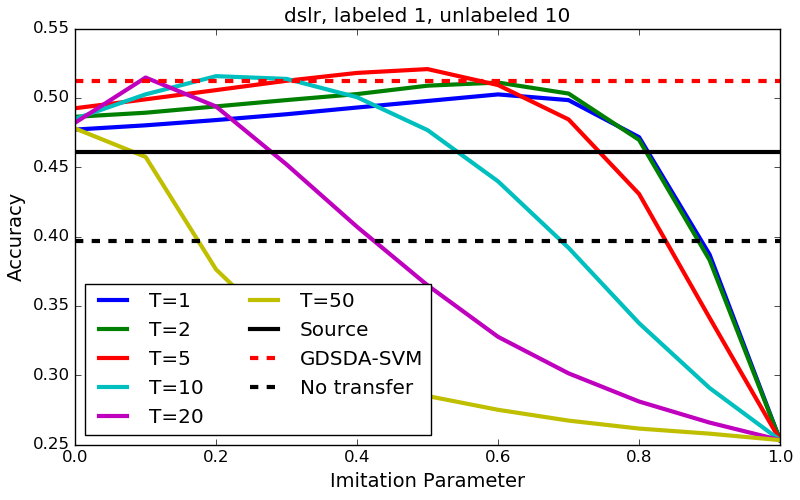
\includegraphics[width=0.2\textwidth]{figure/dslrtoamazonlabeled1unlabeled10.png}}&
\subfloat[D $\rightarrow$ A, 15 unlabeled ]{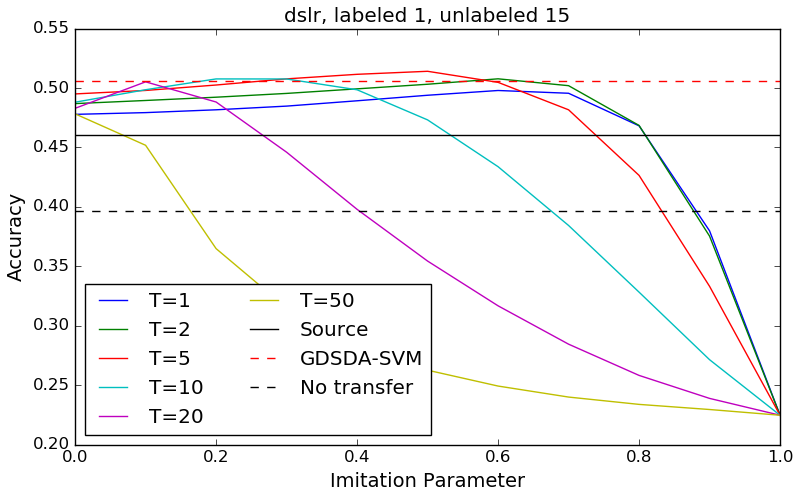
\includegraphics[width=0.2\textwidth]{figure/dslrtoamazonlabeled1unlabeled15.png}}\\
\subfloat[D $\rightarrow$ A, 20 unlabeled ]{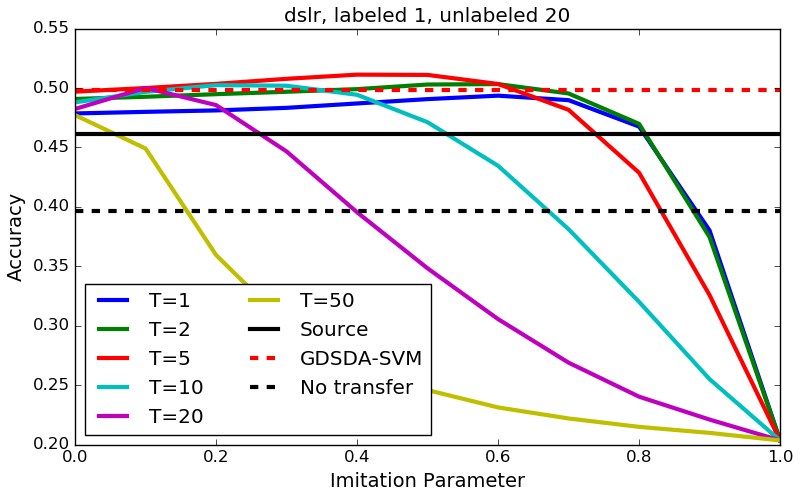
\includegraphics[width=0.2\textwidth]{figure/dslrtoamazonlabeled1unlabeled20.png}}&
\subfloat[W $\rightarrow$ A, 10 unlabeled ]{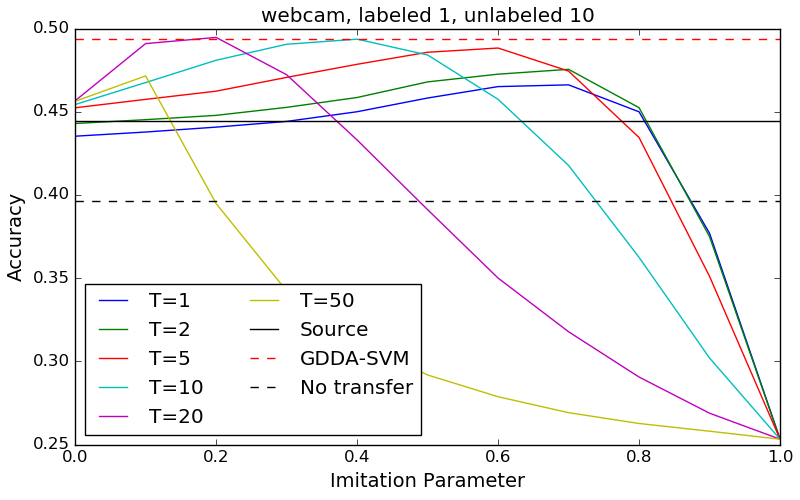
\includegraphics[width=0.2\textwidth]{figure/webcamtoamazonlabeled1unlabeled10.png}}\\
\subfloat[W $\rightarrow$ A, 15 unlabeled ]{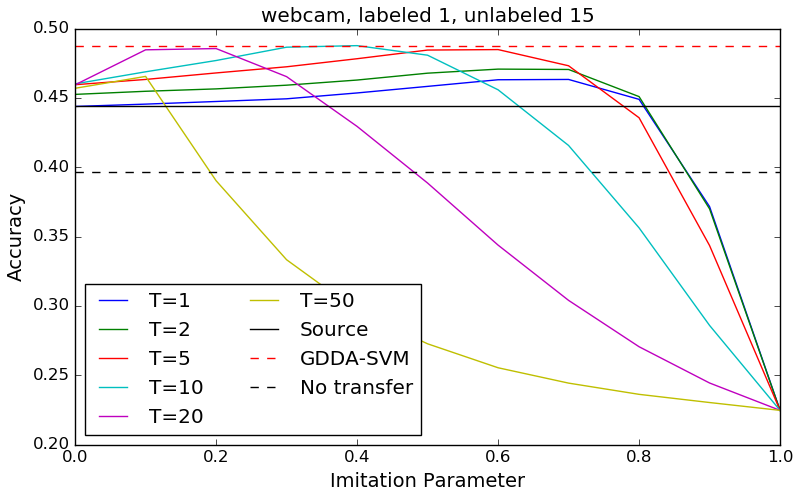
\includegraphics[width=0.2\textwidth]{figure/webcamtoamazonlabeled1unlabeled15.png}}&
\subfloat[W $\rightarrow$ A, 20 unlabeled ]{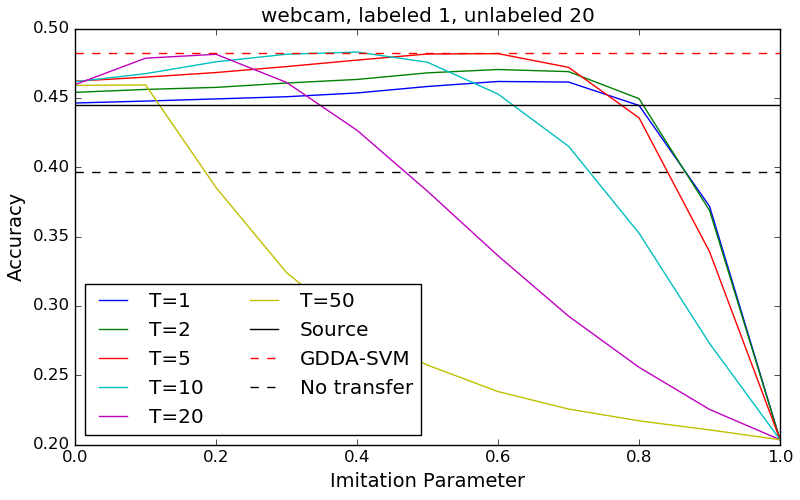
\includegraphics[width=0.2\textwidth]{figure/webcamtoamazonlabeled1unlabeled20.png}}\\
\end{tabular}
\caption{Experiment results on DSLR $\rightarrow$ Amazon and Webcam $\rightarrow$ Amazon when there are just a few labeled examples. The experiments use only 1 labeled example per class. The results of DSLR $\rightarrow$ Amazon and Webcam $\rightarrow$ Amazon are shown in figure (a)-(c) and (d)-(e) respectively. GDSDA-SVM is trained with temperature $T=20$. $\lambda$ on the X-axis denotes the imitation parameter for the hard label and the corresponding imitation parameter for the soft label is set to $1-\lambda$.
}\label{fig:single1}
\end{figure}
\subsection{Multi-Source for Office datasets}
In this experiment, we train the target model for the Amazon, adapting the knowledge from the rest of two source domains, Webcam and DSLR.
We use the identical settings as our single source experiment and perform 2 groups of experiments using 1 labeled and 2 labeled examples per class respectively. We use temperature $T=5$ and the results of multi-source GDSDA-SVM is denoted as SVM\_Multi. Here we use two single source GDSDA-SVMs (SVM\_w and SVM\_d trained with Webcam and DSLR respectively) as the baselines. We also show the best performance of the brutal force results (SVM\_BF). We search temperature in range $T=[1,2,5,10,20,50]$ and each imitation parameter in range $[0,0.1,...,1]$, making sure that their sum equals 1. The experiment results are shown in Figure \ref{fig:multi}.

From the results, we can see that, when we have 2 source domains, SVM\_Multi can still leverage the knowledge effectively and performs better than any single source model. This shows that the imitation parameter estimated by our method can effectively balance the importance of each source to achieve improved performance. SVM\_Multi performs slightly worse than brutal force result in some experiments. However, considering their time complexity (GDSDA-SVM is around 30 times faster than brutal force search), we still think that we still believe that SVM\_Multi is more effectively in real applications.
\begin{figure}
\centering
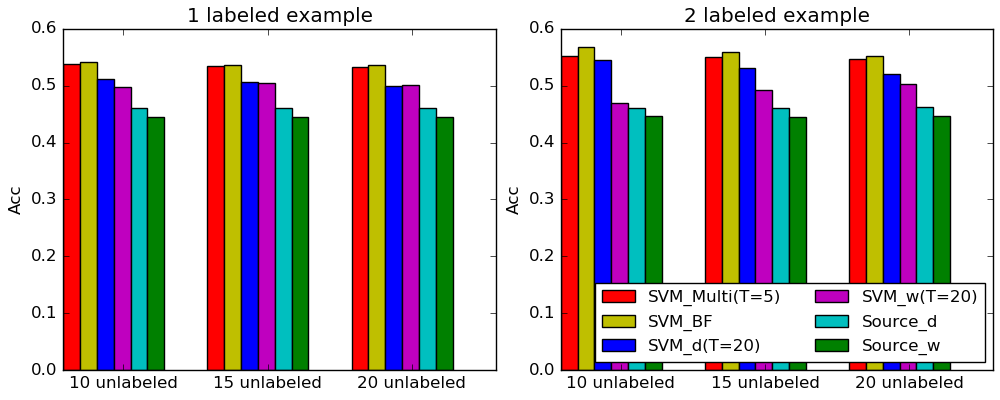
\includegraphics[scale=.3]{figure/cmp.png}
\caption{D+W $\rightarrow$ A, Multi-source results comparison.}\label{fig:multi}
\end{figure}



